\documentclass[11pt,a4paper,titlepage]{article}

\usepackage{geometry}
\geometry{a4paper, margin=1in}

\usepackage{amsmath,amssymb,amsthm}
\usepackage{mathtools}
\usepackage{graphicx}
\usepackage{tikz}
\usepackage{tikz-cd}
\usepackage{booktabs}
\usepackage{tabularx}
\usepackage{fontspec}
\usepackage{hyperref}
\usepackage[svgnames]{xcolor}

\definecolor{navy}{RGB}{15,23,42}
\definecolor{blueaccent}{RGB}{2,132,199}
\definecolor{emerald}{RGB}{16,185,129}
\definecolor{amber}{RGB}{245,158,11}
\definecolor{slate}{RGB}{100,116,139}
\definecolor{indigo}{RGB}{79,70,229}

\hypersetup{
    colorlinks=true,
    linkcolor=blueaccent,
    citecolor=emerald,
    urlcolor=blueaccent
}

% Theorem Environments
\newtheorem{theorem}{Theorem}[section]
\newtheorem{proposition}[theorem]{Proposition}
\newtheorem{lemma}[theorem]{Lemma}
\newtheorem{corollary}[theorem]{Corollary}

\theoremstyle{definition}
\newtheorem{definition}{Definition}[section]
\newtheorem{axiom}{Axiom}[section]
\newtheorem{example}{Example}[section]

\theoremstyle{remark}
\newtheorem{remark}{Remark}[section]

\title{
    \Huge \textbf{Sod Ha-Bechinah:}\\
    \Large Formal Configuration of Relation, Value, Scale, Proportion and Hierarchical Revelation\\[0.5em]
    \large \textbf{סוד הבחינה:}\\
    \large יחס, ערך, קנה־מידה, פרופורציה וגילוי היררכי
}

\author{
    \textbf{WANGA AI Architecture Laboratory}\\
    \small Computational Formalization Group
}

\date{\today}

\begin{document}

\maketitle

\begin{abstract}
This research preprint formalizes the mathematical and computational framework of \emph{Sod Ha-Bechinah} (סוד הבחינה). We model a \emph{Bechinah} (relational aspect/configuration) not as an isolated static object, but as a dynamic configuration vector $B = \operatorname{Bechina}(V,R,S)$ defined over Value ($V$), Relation ($R$), and Scale ($S$). We construct a complete hierarchical configuration space $\Omega_i = (V_i, R_i, S_i, T_i, N_i, G_i, L_i)$ incorporating four computational information layers modeled after \emph{Ta'amim}, \emph{Nekudot}, \emph{Tagin}, and \emph{Otiyot}. We establish rigorous Category-theoretic transition maps $\Phi_i: \Omega_i \to \Omega_{i+1}$ and projection maps $\Pi_i: \Omega_{i+1} \to \Omega_i$, and map these abstractions onto traditional structures including Adam Kadmon ($\mathcal{H} = \{72, 63, 45, 52\}$), Akudim/Nekudim/Berudim, the 231 relational gates ($G_{231} = \binom{22}{2}$), and a 10-node Sefirotic graph network. This paper explicitly separates mathematical definitions from historical textual interpretation and metaphysical claims.
\end{abstract}

\tableofcontents
\newpage

\section*{Notation Reference Table}
\addcontentsline{toc}{section}{Notation Reference Table}

\begin{table}[h!]
\centering
\small
\begin{tabularx}{\textwidth}{l X}
\toprule
\textbf{Symbol} & \textbf{Formal Definition / Description} \\
\midrule
$V$ & Value variable belonging to value space $\mathcal{V}$ \\
$R$ & Relational operator / dependency structure $R \in \mathcal{R}$ \\
$S$ & Scale parameter $S \in \mathbb{R}^+$ \\
$B$ & Bechinah configuration tuple $B = \operatorname{Bechina}(V,R,S)$ \\
$\mathcal{D}$ & Fundamental dimensional space $(P,C,R,\tau)$ (Purpose, Cause, Relation, Time) \\
$\mathcal{I}$ & Four information layers tuple $(T, N, G, L)$ \\
$T, N, G, L$ & Ta'amim, Nekudot, Tagin, Otiyot information resolution layers \\
$\Omega_i$ & Complete configuration state at hierarchical level $i$ \\
$\Phi_i$ & Forward generation / refinement transformation map $\Phi_i: \Omega_i \to \Omega_{i+1}$ \\
$\Pi_i$ & Reverse projection / coarse-graining map $\Pi_i: \Omega_{i+1} \to \Omega_i$ \\
$\mathcal{H}$ & Adam Kadmon numerical representation set $\{72, 63, 45, 52\}$ \\
$G_{231}$ & Set of 231 relational gates $\binom{22}{2}$ \\
$\mathcal{K}$ & Preserved invariant set under scale and structural transformations \\
$\mathfrak{S}(\Omega)$ & Computational integrity canonical serial cryptographic hash \\
\bottomrule
\end{tabularx}
\caption{Canonical Mathematical Symbols and Definitions}
\end{table}

\newpage

\section{Introduction}
\label{sec:introduction}

The concept of \emph{Bechinah} (בחינה, plural: \emph{Bechinot}) occupies a central role in classical Jewish philosophy and Kabbalistic literature, where it denotes an aspect, perspective, or relational modality of revelation. Historically, analysis of \emph{Bechinot} has often been conducted using natural language or metaphysical narrative.

In this work, we present a formal mathematical and computational configuration model titled \textbf{Sod Ha-Bechinah} (סוד הבחינה). Our primary objective is to translate relational intuition into precise mathematical objects, sets, functions, and category-theoretic maps.

We establish three core methodological principles:
\begin{enumerate}
    \item \textbf{Configuration over Isolation}: An aspect ($B$) cannot be modeled in isolation; it emerges strictly from the interaction of Value ($V$), Relation ($R$), and Scale ($S$).
    \item \textbf{Layered Resolution}: Information flows across four distinct resolution layers inspired by \emph{Ta'amim}, \emph{Nekudot}, \emph{Tagin}, and \emph{Otiyot}.
    \item \textbf{Explicit Scope Separation}: Mathematical definitions are strictly distinguished from historical/textual claims and philosophical interpretations.
\end{enumerate}

By doing so, we construct a formal modeling language suitable for computational AI architecture specification.

\section{The Bechinah Mathematical Model}
\label{sec:bechina_model}

We define the fundamental object of study, a \emph{Bechinah}, as a function over a three-dimensional domain space.

\begin{definition}[Value, Relation, Scale Spaces]
Let $\mathcal{V}$ denote a value space, $\mathcal{R}$ denote a space of relational operators, and $\mathcal{S} = \mathbb{R}^+$ denote a positive scalar scale space.
\end{definition}

\begin{definition}[Bechinah Function]
A \emph{Bechinah} $B$ is a configuration map:
\begin{equation}
\boxed{B = \operatorname{Bechina}(V, R, S)}
\end{equation}
where $V \in \mathcal{V}$, $R \in \mathcal{R}$, and $S \in \mathcal{S}$.
\end{definition}

In simple linear approximations, one might consider a multiplicative heuristic for informational content:
\begin{equation}
M = V \cdot R \cdot S
\end{equation}
However, such a simple product fails when relations or scale exhibit non-linear bounds or phase transitions. Therefore, we model general meaningful information ($M$) as a general non-linear operator $F$:
\begin{equation}
M = F(V, R, S)
\end{equation}
This formulation preserves mathematical safety against division by zero and accounts for non-linear scale coupling.

\section{Proportion Logic and Relational Operators}
\label{sec:proportion_logic}

Proportion forms the bedrock of invariant structure. Consider two elements $A, B \in \mathcal{V}$ under a relational ratio operator.

\begin{definition}[Proportional Invariance]
For $A, B, C, D \in \mathcal{V}$ with non-zero denominators, equality of proportion is defined as:
\begin{equation}
A : B = C : D \iff \frac{A}{B} = \frac{C}{D}
\end{equation}
Under a scale transformation $\mathcal{S}_\lambda(x) = \lambda x$ for $\lambda \neq 0$, the ratio remains invariant:
\begin{equation}
\frac{\lambda A}{\lambda B} = \frac{A}{B}
\end{equation}
\end{definition}

This simple property demonstrates how structural information (the ratio $A/B$) is completely preserved even when absolute magnitudes ($A, B \to \lambda A, \lambda B$) undergo global transformation.

\subsection{The Reference / Balancing Third Term}
In formal logic and relational dynamics, two opposing or relative terms $(A, B)$ require a reference condition $C$ to form a balanced relational tuple:
\begin{equation}
(A, B; C)
\end{equation}
where $C$ acts as an invariant boundary condition, reference frame, or balancing mediator.

\section{The Four Fundamental Dimensions}
\label{sec:four_layers}

We define the complete dimensional state space of an architectural configuration as a four-tuple.

\begin{definition}[Fundamental Dimensions Space]
The fundamental dimension space $\mathcal{D}$ is defined as:
\begin{equation}
\mathcal{D} = (P, C, R, \tau)
\end{equation}
where:
\begin{itemize}
    \item $P = \text{Purpose (Finality / Directional Constraint)}$
    \item $C = \text{Cause (Generative Dependency)}$
    \item $R = \text{Relation (Structural Topology)}$
    \item $\tau = \text{Time (Sequential Index)}$
\end{itemize}
\end{definition}

The configuration generation pipeline flows as:
\begin{equation}
P \longrightarrow C \longrightarrow R \longrightarrow \Omega(\tau)
\end{equation}
where $\Omega(\tau)$ represents the system state indexed by sequential time $\tau$.

\begin{proposition}[Finality $\neq$ Temporal Causality]
Purpose ($P$) provides a directional vector field over the state space rather than an efficient temporal cause acting from past to future:
\begin{equation}
\operatorname{Finality}(P) \not\equiv \operatorname{TemporalCause}(C, \tau)
\end{equation}
\end{proposition}

\section{Information Layers: Ta'amim, Nekudot, Tagin, Otiyot}
\label{sec:taamim_nekudot_tagin_otiyot}

Inspired by traditional textual taxonomy, we construct a four-tier computational information encoding model.

\begin{definition}[Information Layers Tuple]
An information encoding state $\mathcal{I}$ is defined as:
\begin{equation}
\mathcal{I} = (T, N, G, L)
\end{equation}
where:
\begin{itemize}
    \item $T = \text{Ta'amim (Syntactic / Prosodic Master Layer)}$
    \item $N = \text{Nekudot (Vocalic / Dynamic Internal State Layer)}$
    \item $G = \text{Tagin (Graphic / Structural Annotation Layer)}$
    \item $L = \text{Otiyot (Discrete Symbolic Carrier / Letter Layer)}$
\end{itemize}
\end{definition}

We map this as an encoding function $\mathcal{E}$ from an abstract state $X$:
\begin{equation}
\mathcal{E} : X \longrightarrow (T, N, G, L)
\end{equation}
Depending on whether the process represents generation (synthesis) or parsing (analysis), the direction flows as:
\begin{equation}
T \xrightarrow{\text{syntactics}} N \xrightarrow{\text{vocalic}} G \xrightarrow{\text{annotations}} L \quad (\text{Encoding})
\end{equation}
or $L \to G \to N \to T$ during decoding.

\section{Adam Kadmon and Numerical Representation}
\label{sec:adam_kadmon}

Traditional Lurianic Kabbalah describes four primary configurations of Adam Kadmon (\emph{AK}) denoted by Gematria expanded name equivalents: $\text{ע"ב}$ (72), $\text{ס"ג}$ (63), $\text{מ"ה}$ (45), and $\text{ב"ן}$ (52).

\begin{definition}[AK Numerical Representation Set]
We formalize the set of primordial configuration indices as:
\begin{equation}
\mathcal{H} = \{ 72, 63, 45, 52 \}
\end{equation}
with a mapping function $H$:
\begin{equation}
H : \{ \text{ע"ב}, \text{ס"ג}, \text{מ"ה}, \text{ב"ן} \} \longrightarrow \mathbb{N}
\end{equation}
\end{definition}

We enforce a strict distinction between symbolic identity and numerical value:
\begin{equation}
\text{Symbol} \neq \text{Number}, \quad \text{but } \operatorname{Representation}(\text{Symbol}) = n \in \mathbb{N}
\end{equation}
The numbers $\{72, 63, 45, 52\}$ serve as formal mathematical dimension tags rather than literal physical quantities.

\section{Hierarchical Level Transformations and Visibility}
\label{sec:transformations}

Configurations exist across discrete hierarchical levels $i \in \mathbb{Z}$.

\begin{definition}[Level State Vector]
A complete level configuration $\Omega_i$ is defined by:
\begin{equation}
\Omega_i = (V_i, R_i, S_i, T_i, N_i, G_i, L_i)
\end{equation}
\end{definition}

Transition between adjacent levels is governed by a forward refinement map $\Phi_i$ and a reverse projection map $\Pi_i$:
\begin{equation}
\boxed{\Omega_i \xrightarrow{\Phi_i} \Omega_{i+1}} \quad \text{(Refinement / Generation)}
\end{equation}
\begin{equation}
\boxed{\Omega_{i+1} \xrightarrow{\Pi_i} \Omega_i} \quad \text{(Projection / Coarse-Graining)}
\end{equation}

Projection is generally lossy ($\Pi_i \neq \Phi_i^{-1}$). We measure information loss via a divergence metric $\mathcal{L}_i$:
\begin{equation}
\mathcal{L}_i = D\left(\Omega_{i+1}, \Psi_i(\Omega_i)\right)
\end{equation}
where $\Psi_i$ is a reconstruction estimator.

\section{The Dynamics of Akudim, Nekudim, and Berudim}
\label{sec:akudim_nekudim_berudim}

We model the classic three-stage structural evolution sequence as a formal system transformation.

\begin{definition}[Tripartite Evolutionary Sequence]
The three structural modes are defined as:
\begin{enumerate}
    \item \textbf{Akudim ($\mathcal{A}_0$)}: Bound / unified single-vessel configuration where all lights reside in a singular vessel.
    \item \textbf{Nekudim ($\mathcal{N}_1$)}: Differentiated / isolated point configuration where discrete isolated vessels lack mutual relation.
    \item \textbf{Berudim ($\mathcal{B}_2$)}: Recombined / balanced matrix configuration featuring inter-vessel channels and proportional reciprocity.
\end{enumerate}
\end{definition}

The formal transformation pipeline is represented as:
\begin{equation}
\mathcal{A}_0 \xrightarrow{\quad \Delta \quad} \mathcal{N}_1 \xrightarrow{\quad \mathcal{T} \quad} \mathcal{B}_2
\end{equation}
where $\Delta$ represents discrete differentiation and $\mathcal{T}$ represents relational reconfiguration and balancing (\emph{Tikun}).

\section{Recursive Models and Whole-Part Relations}
\label{sec:recursive_model}

Hierarchy implies recursion. Let $S_n$ denote the state of system $S$ at depth $n$.

\begin{definition}[Recursive System Iteration]
\begin{equation}
S_{n+1} = F(S_n)
\end{equation}
where $S_n$ contains a set of sub-states:
\begin{equation}
S_n = \{ S_{n-1}^{(1)}, S_{n-1}^{(2)}, \ldots, S_{n-1}^{(k)} \}
\end{equation}
\end{definition}

In complex relational systems, the whole is not a simple linear sum of isolated parts:
\begin{equation}
\operatorname{Whole} = \mathcal{F}(\text{Parts}, \text{Relations}) \neq \sum_{j} \text{Part}_j
\end{equation}
Relational structure carries non-additive mutual information $I(X_1; X_2; \dots; X_k)$ that vanishes if parts are evaluated independently.

\section{Fractal Self-Similarity and Finality Vector}
\label{sec:finality}

Systems that maintain self-similar relational invariants across scaling steps exhibit structural fractal persistence.

\begin{definition}[Structural Invariant Set]
Let $\mathcal{K} = \{ k_1, k_2, \ldots, k_m \}$ be a set of invariants. Under scaling transformation $\Phi$:
\begin{equation}
\Phi(\mathcal{K}) = \mathcal{K}
\end{equation}
The structural similarity between levels $n$ and $n+1$ is preserved if:
\begin{equation}
\Sigma(S_n, S_{n+1}) \approx 1
\end{equation}
\end{definition}

\subsection{Finality as Directional Constraint}
We model Purpose / Finality ($P$) not as a temporal cause, but as a directional vector $\mathbf{F}$ over admissible configurations $\mathcal{D}$:
\begin{equation}
\mathbf{F} : \Omega \longrightarrow \mathcal{D}
\end{equation}
Finality acts as a global optimization constraint guiding local state transitions toward structural equilibrium ($\text{Tikun}$).

\section{Tree of Life Sefirotic Formal Mapping}
\label{sec:tree_of_life_mapping}

We formalize the classical Sefirotic Tree of Life as a directed graph network $\mathcal{G}_{Tree} = (Q, E_{22})$.

\begin{definition}[Sefirotic Node Object]
Each node $Q_i$ ($i \in \{1, \dots, 10\}$) is represented by a structured tuple:
\begin{equation}
Q_i = (M_i, R_i, S_i, V_i, \Phi_i)
\end{equation}
where $M_i$ is station level, $R_i$ is relation set, $S_i$ is scale, $V_i$ is visibility parameter, and $\Phi_i$ is local transition operator.
\end{definition}

\begin{table}[h!]
\centering
\small
\begin{tabular}{c l c c l}
\toprule
\textbf{Node $Q_i$} & \textbf{Traditional Name} & \textbf{Station $M_i$} & \textbf{Scale $S_i$} & \textbf{Category / Role} \\
\midrule
$Q_1$ & Keter & 1 & $1.0$ & Source / Primordial Head \\
$Q_2$ & Chochmah & 2 & $0.9$ & Primary Differentiation \\
$Q_3$ & Binah & 2 & $0.9$ & Structural Receptacle \\
$Q_4$ & Chesed & 3 & $0.7$ & Expansive Flow \\
$Q_5$ & Gevurah & 3 & $0.7$ & Restrictive Bound \\
$Q_6$ & Tiferet & 3 & $0.7$ & Central Harmonizer \\
$Q_7$ & Netzach & 4 & $0.5$ & Active Endurance \\
$Q_8$ & Hod & 4 & $0.5$ & Reflective Echo \\
$Q_9$ & Yesod & 4 & $0.5$ & Foundation Channel \\
$Q_{10}$ & Malchut & 5 & $0.2$ & Physical Manifestation \\
\bottomrule
\end{tabular}
\caption{Mathematical Specification of 10 Sefirotic Nodes}
\end{table}

The 22 connecting channels correspond to edge set $E_{22}$, forming a closed network topology.

\section{Formal Ontology, 22 Letters, and 231 Relational Gates}
\label{sec:formal_ontology}

The symbolic layer of the model incorporates the 22 letters of the Hebrew alphabet as discrete relational generators.

\begin{definition}[22 Symbolic Generators]
Let $\mathcal{L}_{22} = \{ \ell_1, \ell_2, \dots, \ell_{22} \}$ be a set of 22 discrete symbolic elements. Each element $\ell_i$ is represented by:
\begin{equation}
\ell_i = (\sigma_i, \pi_i, \rho_i)
\end{equation}
where $\sigma_i$ is symbolic identity, $\pi_i \in \{1, \dots, 22\}$ is positional index, and $\rho_i$ is relational property.
\end{definition}

\subsection{Combinatorial Derivation of 231 Relational Gates}
Consider pairwise combinations of elements from $\mathcal{L}_{22}$.
\begin{itemize}
    \item Ordered pairs (directed relations): $22 \times 21 = 462$.
    \item Unordered pairs (symmetric relational gates):
    \begin{equation}
    |G_{231}| = \binom{22}{2} = \frac{22 \times 21}{2} = 231
    \end{equation}
\end{itemize}

\begin{definition}[231 Relational Gate Set]
The set of 231 relational gates $G_{231}$ is defined precisely as the set of all unordered 2-element subsets:
\begin{equation}
\boxed{g_{ij} = \{ \ell_i, \ell_j \} \quad \text{for } 1 \le i < j \le 22}
\end{equation}
\end{definition}

\subsection{Computational Integrity Seal}
We establish computational verification of a state configuration $\Omega$ via a canonical serialization hash $\mathfrak{S}(\Omega)$:
\begin{equation}
\mathfrak{S}(\Omega) = \operatorname{Hash}\Big(\operatorname{CanonicalSerialize}(\Omega)\Big)
\end{equation}
This seal verifies computational integrity ($\operatorname{Integrity} \neq \operatorname{Truth}$).

\section{Conclusion and Formal Limitations}
\label{sec:conclusion}

In this paper, we have presented a formal configuration research model for \textbf{Sod Ha-Bechinah} (סוד הבחינה).

We have established:
\begin{enumerate}
    \item The core relational model $B = \operatorname{Bechina}(V, R, S)$.
    \item The four fundamental dimensions $\mathcal{D} = (P, C, R, \tau)$ and information encoding layers $\mathcal{I} = (T, N, G, L)$.
    \item Hierarchical state vectors $\Omega_i = (V_i, R_i, S_i, T_i, N_i, G_i, L_i)$ with refinement maps $\Phi_i$ and projection maps $\Pi_i$.
    \item Mathematical formalizations for Adam Kadmon Gematria sets $\mathcal{H} = \{72, 63, 45, 52\}$, Akudim/Nekudim/Berudim transformations, Sefirotic graph networks, and the 231 relational gates $G_{231} = \binom{22}{2}$.
\end{enumerate}

\subsection*{Formal Limitations}
We conclude with an explicit methodological boundary:
\begin{quote}
This project does not claim to mathematically prove metaphysical or theological propositions. Instead, it constructs a formal, self-consistent modeling language in which relations, scales, configurations, information layers, transformations, and hierarchical visibility can be represented rigorously and implemented computationally.
\end{quote}


\appendix
\section{TikZ Structural Diagrams}
\label{appendix:tikz}

\subsection{Master Hierarchy Diagram}
\begin{figure}[h!]
\centering
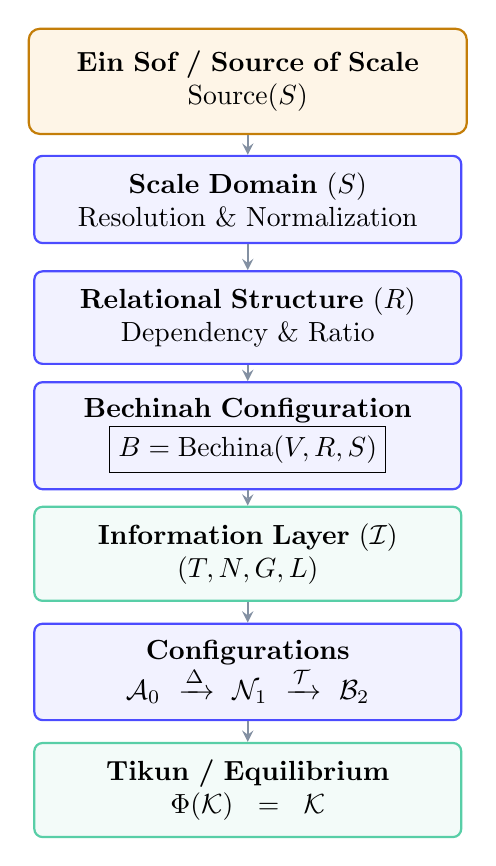
\begin{tikzpicture}[node distance=1.5cm, auto, >=stealth,
    block/.style={rectangle, draw=blue!70, fill=blue!5, thick, inner sep=6pt, text width=5cm, align=center, rounded corners=3pt},
    source/.style={rectangle, draw=amber!80!black, fill=amber!10, thick, inner sep=8pt, text width=5cm, align=center, rounded corners=4pt},
    info/.style={rectangle, draw=emerald!70, fill=emerald!5, thick, inner sep=6pt, text width=5cm, align=center, rounded corners=3pt},
    edge/.style={->, thick, draw=slate!80}]

\node [source] (einsof) {\textbf{Ein Sof / Source of Scale}\\$\operatorname{Source}(S)$};
\node [block, below of=einsof] (scale) {\textbf{Scale Domain} ($S$)\\Resolution \& Normalization};
\node [block, below of=scale] (relation) {\textbf{Relational Structure} ($R$)\\Dependency \& Ratio};
\node [block, below of=relation] (bechina) {\textbf{Bechinah Configuration}\\$\boxed{B = \operatorname{Bechina}(V,R,S)}$};
\node [info, below of=bechina] (info_layer) {\textbf{Information Layer} ($\mathcal{I}$)\\$(T, N, G, L)$};
\node [block, below of=info_layer] (anb) {\textbf{Configurations}\\$\mathcal{A}_0 \xrightarrow{\Delta} \mathcal{N}_1 \xrightarrow{\mathcal{T}} \mathcal{B}_2$};
\node [info, below of=anb] (tikun) {\textbf{Tikun / Equilibrium}\\$\Phi(\mathcal{K}) = \mathcal{K}$};

\draw [edge] (einsof) -- (scale);
\draw [edge] (scale) -- (relation);
\draw [edge] (relation) -- (bechina);
\draw [edge] (bechina) -- (info_layer);
\draw [edge] (info_layer) -- (anb);
\draw [edge] (anb) -- (tikun);

\end{tikzpicture}

\caption{Master Hierarchy of Scale, Relation, and Configuration}
\end{figure}

\subsection{Four Information Layers Diagram}
\begin{figure}[h!]
\centering
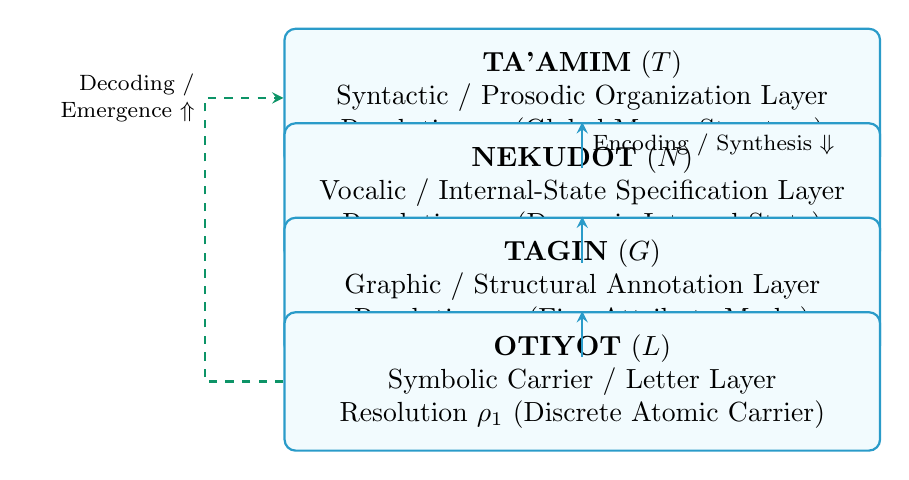
\begin{tikzpicture}[node distance=1.2cm, auto, >=stealth,
    layer/.style={rectangle, draw=cyan!80!black, fill=cyan!5, thick, inner sep=8pt, text width=7cm, align=center, rounded corners=4pt},
    edge/.style={->, thick, draw=cyan!80!black}]

\node [layer] (taamim) {\textbf{TA'AMIM} ($T$)\\Syntactic / Prosodic Organization Layer\\$\text{Resolution } \rho_4 \text{ (Global Macro-Structure)}$};
\node [layer, below of=taamim] (nekudot) {\textbf{NEKUDOT} ($N$)\\Vocalic / Internal-State Specification Layer\\$\text{Resolution } \rho_3 \text{ (Dynamic Internal State)}$};
\node [layer, below of=nekudot] (tagin) {\textbf{TAGIN} ($G$)\\Graphic / Structural Annotation Layer\\$\text{Resolution } \rho_2 \text{ (Fine Attribute Marks)}$};
\node [layer, below of=tagin] (otiyot) {\textbf{OTIYOT} ($L$)\\Symbolic Carrier / Letter Layer\\$\text{Resolution } \rho_1 \text{ (Discrete Atomic Carrier)}$};

\draw [edge] (taamim) -- node[right, font=\footnotesize] {Encoding / Synthesis $\Downarrow$} (nekudot);
\draw [edge] (nekudot) -- (tagin);
\draw [edge] (tagin) -- (otiyot);

\draw [edge, dashed, draw=emerald!80!black] (otiyot.west) -- ++(-1,0) |- node[left, font=\footnotesize, text width=2cm, align=right] {Decoding / Emergence $\Uparrow$} (taamim.west);

\end{tikzpicture}

\caption{Encoding and Decoding Directions across Information Layers}
\end{figure}

\subsection{Transformation Between Levels}
\begin{figure}[h!]
\centering
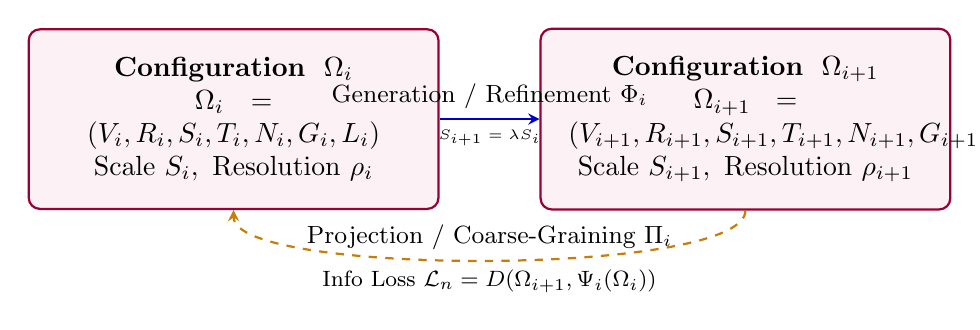
\begin{tikzpicture}[node distance=2.5cm, auto, >=stealth,
    state/.style={rectangle, draw=purple!80!black, fill=purple!5, thick, inner sep=10pt, text width=4.5cm, align=center, rounded corners=4pt},
    arrow/.style={->, thick, draw=blue!80!black},
    proj/.style={->, thick, dashed, draw=amber!80!black}]

\node [state] (om_i) {\textbf{Configuration } $\Omega_i$\\$\Omega_i = (V_i, R_i, S_i, T_i, N_i, G_i, L_i)$\\$\text{Scale } S_i, \text{ Resolution } \rho_i$};
\node [state, right of=om_i, node distance=6.5cm] (om_i1) {\textbf{Configuration } $\Omega_{i+1}$\\$\Omega_{i+1} = (V_{i+1}, R_{i+1}, S_{i+1}, T_{i+1}, N_{i+1}, G_{i+1}, L_{i+1})$\\$\text{Scale } S_{i+1}, \text{ Resolution } \rho_{i+1}$};

\draw [arrow] (om_i) -- node[above, font=\small] {Generation / Refinement $\Phi_i$} node[below, font=\tiny] {$S_{i+1} = \lambda S_i$} (om_i1);
\draw [proj] (om_i1) .. controls +(down:2cm) and +(down:2cm) .. node[above, font=\small] {Projection / Coarse-Graining $\Pi_i$} node[below, font=\footnotesize] {Info Loss $\mathcal{L}_n = D(\Omega_{i+1}, \Psi_i(\Omega_i))$} (om_i);

\end{tikzpicture}

\caption{Forward Refinement $\Phi_i$ and Projection Map $\Pi_i$ with Information Loss}
\end{figure}

\subsection{Tree of Life Sefirotic Mapping}
\begin{figure}[h!]
\centering
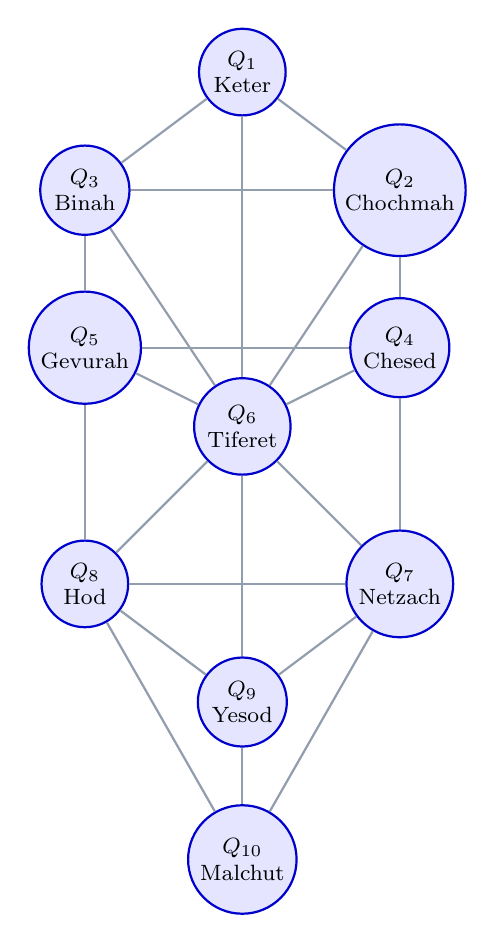
\begin{tikzpicture}[
    sefira/.style={circle, draw=blue!80!black, fill=blue!10, thick, inner sep=2pt, minimum size=1.1cm, align=center, font=\footnotesize},
    edge/.style={-, thick, draw=slate!70}
]

% Nodes
\node[sefira] (keter) at (0, 4.5) {$Q_1$\\Keter};
\node[sefira] (chochmah) at (2, 3) {$Q_2$\\Chochmah};
\node[sefira] (binah) at (-2, 3) {$Q_3$\\Binah};
\node[sefira] (chesed) at (2, 1) {$Q_4$\\Chesed};
\node[sefira] (gevurah) at (-2, 1) {$Q_5$\\Gevurah};
\node[sefira] (tiferet) at (0, 0) {$Q_6$\\Tiferet};
\node[sefira] (netzach) at (2, -2) {$Q_7$\\Netzach};
\node[sefira] (hod) at (-2, -2) {$Q_8$\\Hod};
\node[sefira] (yesod) at (0, -3.5) {$Q_9$\\Yesod};
\node[sefira] (malchut) at (0, -5.5) {$Q_{10}$\\Malchut};

% Edges (3 Columns / 22 Channels)
\draw[edge] (keter) -- (chochmah);
\draw[edge] (keter) -- (binah);
\draw[edge] (chochmah) -- (binah);

\draw[edge] (chochmah) -- (chesed);
\draw[edge] (binah) -- (gevurah);

\draw[edge] (keter) -- (tiferet);
\draw[edge] (chochmah) -- (tiferet);
\draw[edge] (binah) -- (tiferet);

\draw[edge] (chesed) -- (gevurah);
\draw[edge] (chesed) -- (tiferet);
\draw[edge] (gevurah) -- (tiferet);

\draw[edge] (chesed) -- (netzach);
\draw[edge] (gevurah) -- (hod);

\draw[edge] (tiferet) -- (netzach);
\draw[edge] (tiferet) -- (hod);
\draw[edge] (tiferet) -- (yesod);

\draw[edge] (netzach) -- (hod);
\draw[edge] (netzach) -- (yesod);
\draw[edge] (hod) -- (yesod);

\draw[edge] (netzach) -- (malchut);
\draw[edge] (hod) -- (malchut);
\draw[edge] (yesod) -- (malchut);

\end{tikzpicture}

\caption{Mathematical Graph Topology of Sefirotic Nodes and Channels}
\end{figure}

\subsection{Recursive Structural Invariance}
\begin{figure}[h!]
\centering
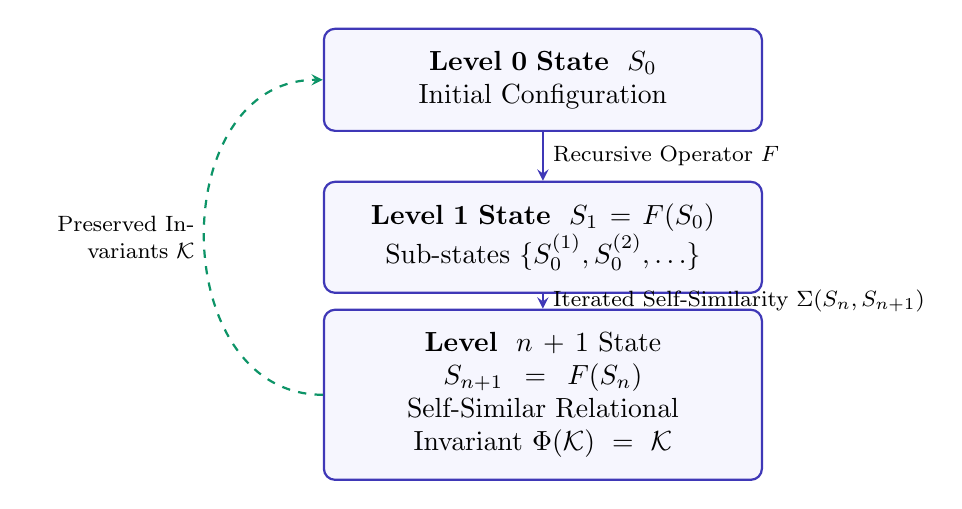
\begin{tikzpicture}[node distance=2cm, auto, >=stealth,
    box/.style={rectangle, draw=indigo!80!black, fill=indigo!5, thick, inner sep=8pt, text width=5cm, align=center, rounded corners=4pt},
    edge/.style={->, thick, draw=indigo!80!black}]

\node [box] (s0) {\textbf{Level 0 State } $S_0$\\Initial Configuration};
\node [box, below of=s0] (s1) {\textbf{Level 1 State } $S_1 = F(S_0)$\\$\text{Sub-states } \{S_0^{(1)}, S_0^{(2)}, \ldots\}$};
\node [box, below of=s1] (s2) {\textbf{Level } $n+1$ State $S_{n+1} = F(S_n)$\\Self-Similar Relational Invariant $\Phi(\mathcal{K}) = \mathcal{K}$};

\draw [edge] (s0) -- node[right, font=\footnotesize] {Recursive Operator $F$} (s1);
\draw [edge] (s1) -- node[right, font=\footnotesize] {Iterated Self-Similarity $\Sigma(S_n, S_{n+1})$} (s2);

\draw [edge, dashed, draw=emerald!80!black] (s2.west) .. controls +(-2,0) and +(-2,0) .. node[left, font=\footnotesize, text width=2cm, align=right] {Preserved Invariants $\mathcal{K}$} (s0.west);

\end{tikzpicture}

\caption{Recursive Self-Similarity and Preserved Invariant Set $\mathcal{K}$}
\end{figure}

\nocite{*}
\bibliographystyle{plain}
\bibliography{bibliography}

\end{document}
